\documentclass[12pt]{article}

\usepackage{hyperref} % гиперссылки

\usepackage{tikz} % картинки в tikz
\usetikzlibrary{arrows.meta} % tikz-прибамбас для рисовки стрелочек подлиннее

\usepackage{microtype} % свешивание пунктуации

\usepackage{array} % для столбцов фиксированной ширины

\usepackage{indentfirst} % отступ в первом параграфе

\usepackage{sectsty} % для центрирования названий частей
\allsectionsfont{\centering}

\usepackage{amsmath} % куча стандартных математических плюшек
\usepackage{amssymb} % символы
\usepackage{amsthm} % теоремки

\usepackage{comment} % добавление длинных комментариев

\usepackage[top=2cm, left=1.2cm, right=1.2cm, bottom=2cm]{geometry} % размер текста на странице

\usepackage{lastpage} % чтобы узнать номер последней страницы

\usepackage{enumitem} % дополнительные плюшки для списков
%  например \begin{enumerate}[resume] позволяет продолжить нумерацию в новом списке

\usepackage{caption} % что-то делает с подписями рисунков :)

\usepackage{qcircuit} % для рисовки квантовых диаграмм
\usepackage{physics} % бракеты

\usepackage{answers} % разделение условий и ответов в упражнениях


\usepackage{fancyhdr} % весёлые колонтитулы
\pagestyle{fancy}
\lhead{Квантовые вычисления}
\chead{}
\rhead{КЛШ-2018}
\lfoot{}
\cfoot{}
\rfoot{\thepage/\pageref{LastPage}}
\renewcommand{\headrulewidth}{0.4pt}
\renewcommand{\footrulewidth}{0.4pt}



\usepackage{todonotes} % для вставки в документ заметок о том, что осталось сделать
% \todo{Здесь надо коэффициенты исправить}
% \missingfigure{Здесь будет Последний день Помпеи}
% \listoftodos — печатает все поставленные \todo'шки



\usepackage{booktabs} % красивые таблицы
% заповеди из докупентации:
% 1. Не используйте вертикальные линни
% 2. Не используйте двойные линии
% 3. Единицы измерения - в шапку таблицы
% 4. Не сокращайте .1 вместо 0.1
% 5. Повторяющееся значение повторяйте, а не говорите "то же"



\usepackage{fontspec} % что-то про шрифты?
\usepackage{polyglossia} % русификация xelatex

\setmainlanguage{russian}
\setotherlanguages{english}

% download "Linux Libertine" fonts:
% http://www.linuxlibertine.org/index.php?id=91&L=1
\setmainfont{Linux Libertine O} % or Helvetica, Arial, Cambria
% why do we need \newfontfamily:
% http://tex.stackexchange.com/questions/91507/
\newfontfamily{\cyrillicfonttt}{Linux Libertine O}

\AddEnumerateCounter{\asbuk}{\russian@alph}{щ} % для списков с русскими буквами
\setlist[enumerate, 2]{label=\asbuk*),ref=\asbuk*}

%% эконометрические сокращения
\DeclareMathOperator{\Cov}{Cov}
\DeclareMathOperator{\Arg}{Arg}
\DeclareMathOperator{\Corr}{Corr}
\DeclareMathOperator{\Var}{Var}
\DeclareMathOperator{\E}{\mathbb{E}}
\def \hb{\hat{\beta}}
\def \hs{\hat{\sigma}}
\def \htheta{\hat{\theta}}
\def \s{\sigma}
\def \hy{\hat{y}}
\def \hY{\hat{Y}}
\def \v1{\vec{1}}
\def \e{\varepsilon}
\def \he{\hat{\e}}
\def \z{z}
\def \hVar{\widehat{\Var}}
\def \hCorr{\widehat{\Corr}}
\def \hCov{\widehat{\Cov}}
\def \cN{\mathcal{N}}
\let\P\relax
\DeclareMathOperator{\P}{\mathbb{P}}



\usepackage[bibencoding = auto,
backend = biber,
sorting = none,
style=alphabetic]{biblatex}

\addbibresource{em1_pset_v2.bib}



% делаем короче интервал в списках
\setlength{\itemsep}{0pt}
\setlength{\parskip}{0pt}
\setlength{\parsep}{0pt}




\Newassociation{sol}{solution}{solution_file}
% sol --- имя окружения внутри задач
% solution --- имя окружения внутри solution_file
% solution_file --- имя файла в который будет идти запись решений
% можно изменить далее по ходу
\Opensolutionfile{solution_file}[all_solutions]
% в квадратных скобках фактическое имя файла

% магия для автоматических гиперссылок задача-решение
\newlist{myenum}{enumerate}{3}
% \newcounter{problem}[chapter] % нумерация задач внутри глав
\newcounter{problem}[section]

\newenvironment{problem}%
{%
\refstepcounter{problem}%
%  hyperlink to solution
     \hypertarget{problem:{\thesection.\theproblem}}{} % нумерация внутри глав
     % \hypertarget{problem:{\theproblem}}{}
     \Writetofile{solution_file}{\protect\hypertarget{soln:\thesection.\theproblem}{}}
     %\Writetofile{solution_file}{\protect\hypertarget{soln:\theproblem}{}}
     \begin{myenum}[label=\bfseries\protect\hyperlink{soln:\thesection.\theproblem}{\thesection.\theproblem},ref=\thesection.\theproblem]
     % \begin{myenum}[label=\bfseries\protect\hyperlink{soln:\theproblem}{\theproblem},ref=\theproblem]
     \item%
    }%
    {%
    \end{myenum}}
% для гиперссылок обратно надо переопределять окружение
% это происходит непосредственно перед подключением файла с решениями



\theoremstyle{definition}
\newtheorem{definition}{Определение}



\begin{document}

\tableofcontents{}

\section*{Цель}

Рассказать про квантовые вычисления девятиклассникам.
Дойти до алгоритма Гровера с нуля, включая рассказ про вероятности и комплексные числа.

Спорные моменты:

\begin{itemize}
  \item полный отказ от матриц, только обозначения Дирака;
  \item что делать с экспонентой $e$?
\end{itemize}


\newpage
\section{Посади дерево!}

\begin{definition}
$A$ — событие, $\P(A)$ — вероятность события $A$.

$X$ — случайная величина, $\E(X)$ — математическое ожидание величины $X$.
\end{definition}

\begin{problem}
В вазе пять неотличимых с виду конфет.
Две без ореха и три — с орехом. Маша ест конфеты выбирая их наугад до тех пор,
пока не съест первую конфету с орехом. Обозначим $X$ — число съеденных конфет.
Найди вероятности $\P(X=2)$, $\P(X>1)$ и ожидание $\E(X)$.


\begin{sol}
  $\P(X=1)=3/5$, $\P(X=2)=3/10$, $\P(X=3)=1/10$, $\E(X)=1.5$
\end{sol}
\end{problem}

\begin{problem}
В коробке находится четыре внешне одинаковые лампочки,  две из них исправны.
Лампочки извлекают из коробки по одной до тех пор, пока не будут извлечены обе исправные.
\begin{enumerate}
\item Какова вероятность того, что опыт закончится извлечением трёх лампочек?
\item Каково ожидаемое количество извлеченных лампочек?
\end{enumerate}

\begin{sol}
\end{sol}
\end{problem}

\begin{problem}
Маша подкидывает монетку. Если она выпадает орлом, то Маша подкидывает монетку ещё один раз,
если решкой — то ещё два раза. После этого Маша идёт в кино!
Пусть $X$ — количество выпавших орлов.

Найди вероятности $\P(X=0)$, $\P(X=1)$ и ожидание $\E(X)$.

\begin{sol}
\end{sol}
\end{problem}

\begin{problem}
Две команды равной силы играют в волейбол до трёх побед одной из них,
не обязательно подряд. Ничья невозможна. Из-за равенства сил будем считать,
что вероятность победы каждой равна $0.5$. Величина $N$ — количество сыгранных партий.

Составьте табличку возможных значений $N$ с их вероятностями.

Найди вероятность $\P(N \text{ — чётное})$ и ожидание $\E(N)$.


\begin{sol}
   N 3 4 5

  2/8 3/8 3/8
\end{sol}
\end{problem}

\begin{problem}
Какова вероятность того, что у 13 человек не будет ни одного совпадения дней рождений?
\begin{sol}

\end{sol}
\end{problem}


\section{К чёрту условности!}

\begin{definition}
Условная вероятность события $A$ при условии, что событие $B$ произошло,
\[
\P(A|B) = \frac{\P(A \cap B)}{\P(B)}
\]
\end{definition}




\begin{problem}
В городе примерно 4\% такси зелёного цвета и остальные жёлтые. Свидетель путает цвет на показаниях в суде с вероятностью 10\%.

\begin{enumerate}
\item Какова вероятность того, свидетель скажет, что видел зелёное такси?
\item Какова вероятность того, свидетель ошибётся?
\item Какова вероятность того, что такси было зелёным, если свидетель говорит, что оно было зелёным?
\item Какова вероятность того, что такси было жёлтым, если свидетель говорит, что оно было жёлтым?
\end{enumerate}
\end{problem}


\begin{problem}
У тети Маши — двое детей, один старше другого. Предположим, что вероятности рождения мальчика и девочки равны и не зависят от дня недели, а пол первого и второго ребенка независимы. Для каждой из ситуаций найдите условную вероятность того, что у тёти Маши есть дети обоих полов.
\begin{enumerate}
\item Известно, что старший ребенок — мальчик.
\item Тетя Маша наугад выбирает одного своего
ребенка и посылает к тете Оле, вернуть метлу. Это оказывается мальчик.
\item На вопрос: «А правда ли тётя Маша, что у Вас есть хотя бы один сын?» тётя Маша ответила: «Да».
\item На вопрос: «А правда ли тётя Маша, что у Вас есть хотя бы один сын, родившийся в пятницу?» тётя Маша ответила: «Да».
\end{enumerate}
\end{problem}


\begin{problem}
Ты смертельно болен. Спасти тебя может только один вид  целебной лягушки.
Целебны у этого вида только самцы. Самцы и самки встречаются равновероятно.
Ты на дороге и предельно ослаб и можешь проползти лишь 100 метров.
Справа в 100 метров аж две лягушки целебного вида, издалека неясно кто.
От двух лягушек в твою сторону дует ветер, поэтому ты можешь их слышать.

Каковы твои шансы на спасение в каждом из случаев?
\begin{enumerate}
  \item Cамцы и самки квакают одинаково, со стороны правых двух лягушек ты слышишь кваканье.
  \item Самки квакают, самцы — нет, со стороны правых двух лягушек ты слышишь кваканье, но не разобрать, одной лягушки или двух.
  \item Самцы и самки квакают по разному, но одинаково часто. Ты слышишь отдельный квак одной из двух лягушек справа и это квак самки.
\end{enumerate}
\end{problem}

\begin{problem} Monty-Hall

Есть три закрытых двери. За двумя из них — по козе, за третьей автомобиль. Ты выбираешь одну из дверей. Допустим, ты выбрал дверь А. Ведущий шоу открывает дверь B и за ней нет автомобиля.
В этот момент ведущий предлагает тебе изменить выбор двери.

Имеет ли смысл изменить выбор в каждой из трёх ситуаций?
\begin{enumerate}
  \item Ведущий выбирал одну из трёх дверей равновероятно.
  \item Ведущий выбирал одну из двух дверей не выбранных тобой равновероятно.
  \item Ведущий выбирал дверь без машины и не совпадающую с твоей.
\end{enumerate}
\end{problem}




\newpage
\section{Не комплексуй без комплексных чисел}

\begin{definition}
Комплексное число — это вектор на плоскости.

\begin{enumerate}
  \item Длина вектора — модуль комплексного числа, $|z|$.
  \item Угол между вектором и горизонатльной осью — аргумента комплексного числа, $\Arg z$.
  \item Горизонтальная составляющая вектора — действительная часть, $\Re z$.
  \item Вертикальная составляющая вектора — мнимая часть, $\Im z$.
\end{enumerate}

\begin{problem}
Для комплексных чисел $1+i$ и $3+4i$ найди $|z|$, $\Arg z$, $\Re z$, $\Im z$. Нарисуй числа $1+i$ и $3+4i$.

\begin{sol}
\end{sol}
\end{problem}


Действия:
\begin{enumerate}
  \item Сложение комплексных чисел — сложение векторов.
  \item Умножение комплексных чисел — длины векторов умножаются, аргументы складываются.
  \item Сопряжение $z^*$ комплексного числа — отражение относительно горизонтальной оси.
\end{enumerate}
\end{definition}


\begin{problem}
Базируясь на геометрическом определении умножения, ответь на вопросы:

\begin{enumerate}
  \item Чему равняется $(1+i)^2$? $(1+i)^{43}$?
  \item Почему $i^2=-1$?
  \item Чему равняется произведение произвольного комплексного числа  $z=a+bi$ на $i$?
  \item Нарисуй процесс умножение произвольного $z=a+bi$ на $3+4i$. Почему $(3+4i)z = 3z + 4iz$?
\end{enumerate}

\begin{sol}
\end{sol}
\end{problem}


\begin{problem}

\begin{enumerate}
  \item У комплексного числа $w = \sqrt{11} + 5i$ найди $|w|$, $|w|^2$, $\Arg w$, $\Re w$, $\Im w$, $w^*$, $ww^*$.
  \item Найди $(3+5i) \cdot (3+3i)$, $(1+i)/(1-i)$,
  \item Найди $(\sqrt{3}+i)^{43}$, $(1-i)^{2018}$;
  \item Найди $(\cos (20^{\circ}) + i \sin (20^{\circ})) \cdot (\cos (10^{\circ}) + i \sin (10^{\circ}))$;
  \item Найди $(\cos (20^{\circ}) + i \sin (20^{\circ})) / (\cos (10^{\circ}) + i \sin (10^{\circ}))$;
\end{enumerate}

\begin{sol}
\end{sol}
\end{problem}


\begin{problem}
Реши уравнения $z^2 + 6z + 10 = 0$, $z^6 = 64$, $(z-1) / (z + 1) = 1 + 3i$.
\begin{sol}
\end{sol}
\end{problem}

\begin{problem}
  Бесконечно живущая черепаха за первый день проходит 10 км на север.
  Затем каждый день она поворачивает на $90^{\circ}$ налево и
  снижает скорость на 20\%. К какой точке она приближается?

  К какой точке стремится черепах, если она поворачивает на $60^{\circ}$?
\begin{sol}
\end{sol}
\end{problem}




\begin{problem}
  Найди сумму углов между векторами и горизонтальной осью.


  \begin{minipage}{0.8\textwidth}
  \begin{center}
  \begin{tikzpicture}
  \draw (0,0) -- (4,0);
  \draw (0,1) -- (4,1);
  \draw (0,2) -- (4,2);
  \draw (0,0) -- (0,2);
  \draw (1,0) -- (1,2);
  \draw (2,0) -- (2,2);
  \draw (3,0) -- (3,2);
  \draw (4,0) -- (4,2);
  \draw[-{Latex[length=5mm, width=2mm]}] (0,0) -- (4,2);
  \draw[-{Latex[length=5mm, width=2mm]}] (0,0) -- (3,1);
  \end{tikzpicture}
  \end{center}
  \end{minipage}
\begin{sol}
  $(4+2i)(3+i) = 10 + 10i$, $\pi/4$.
\end{sol}
\end{problem}



\begin{problem}
На плоскости нарисована кошечка. Что прозойдет с кошечкой,
если каждую точку кошечки домножить на комплексное число $1/\sqrt{2} + i/\sqrt{2}$?
\begin{sol}
  Кошка повернётся на $\pi/4$ против часовой стрелки относительно начала координат
\end{sol}
\end{problem}


\newpage
\section{Ноль без палочки}


\begin{minipage}{0.8\textwidth}
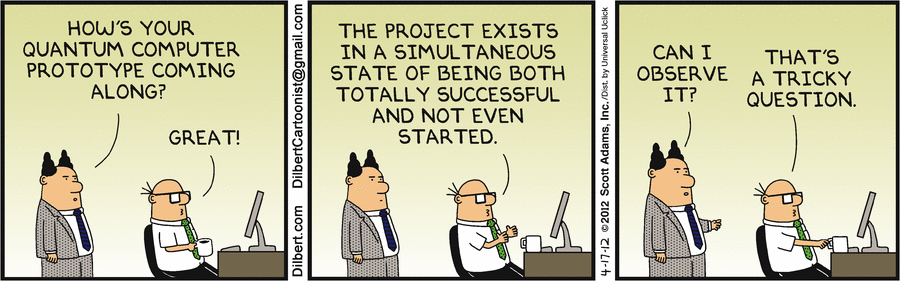
\includegraphics[width=\textwidth]{image/dilbert_quantum_prototype.png}
\end{minipage}


\begin{problem}
  Составь таблицу истинности для следующих классических схем:

  (тут от фонаря схема примерно пятью элементами)
\begin{sol}

\end{sol}
\end{problem}




\begin{problem}
С помощью классических логических элементов $NOT$, $AND$, $OR$ реализуй схемы:
\begin{enumerate}
  \item $OR$ с пятью входами: выдаёт на выходе 1, если хотя бы один из входов
  равен 1, и выдаёт 0 иначе.
  \item исключающее ИЛИ, $XOR$;
  \item сумматор для двух двухбитных чисел с трёхбитным выходом.
\end{enumerate}
\begin{sol}

\end{sol}
\end{problem}


\begin{definition}
Кубит может находиться в бесконечном количестве состояний
\[
\ket{q} = \alpha_0 \ket{0} + \alpha_1 \ket{1}
\]

Амплитуды $\alpha_0$ и $\alpha_1$ — это комплексные числа удовлетворяющие соотношению $|\alpha_0|^2 + |\alpha_1|^2 = 1$.

Также кубит можно записать в столбик:
\[
\ket{q} = \alpha_0 \ket{0} + \alpha_1 \ket{1} =
\begin{pmatrix}
  \alpha_0 \\
  \alpha_1 \\
\end{pmatrix}
\]


Если измерить кубит $\ket{q} = \alpha_0 \ket{0} + \alpha_1 \ket{1}$
в базисе $\ket{0}$ и $\ket{1}$, то он
перейдёт в детерминистическое состояние $\ket{0}$ с вероятностью $|\alpha_0|^2$
и в детерминистическое состояние $\ket{1}$ с вероятностью $|\alpha_1|^2$.
\end{definition}


\begin{problem}
  Для каждого выражения определи, является ли оно честным и благородным кубитом.
  Для кубитов определи вероятности пронаблюдать их в состояниях $\ket{0}$ и $\ket{1}$:
  \begin{enumerate}
    \item $\frac{1}{2}\ket{0} + \frac{1}{2}\ket{1}$;
    \item $\frac{1}{\sqrt{2}}\ket{0} + \frac{i}{\sqrt{2}}\ket{1}$;
    \item $\ket{0} + \ket{1}$;
    \item $\frac{\sqrt{3}}{2}\ket{0} - \frac{1}{2}\ket{1}$;
    \item $\ket{1}$;
    \item $\cos 10^{\circ} \ket{0} + (\cos 12^{\circ} + i \sin 12^{\circ})\sin 12^{\circ} \ket{1}$;
    \item $\cos 15^{\circ} \ket{0} + (\cos 12^{\circ} + i \sin 12^{\circ})\sin 15^{\circ} \ket{1}$;
    \item $(\cos 35^{\circ} + i \sin 35^{\circ})\cos 45^{\circ} \ket{0} + (\cos 22^{\circ} + i \sin 22^{\circ})\sin 45^{\circ} \ket{1}$;
  \end{enumerate}

\begin{sol}

\end{sol}
\end{problem}

\begin{problem}
Два важных кубита, это $\ket{+} = \frac{1}{\sqrt{2}}(\ket{0} + \ket{1})$ и  $\ket{-} = \frac{1}{\sqrt{2}}(\ket{0} - \ket{1})$.

\begin{enumerate}
  \item У Дианы в одной коробке 1000 кубитов $\ket{+}$, а в другой —
  1000 кубитов $\frac{\sqrt{3}}{2}\ket{0} + \frac{1}{2}\ket{1}$.
  К сожалению, коробки не подписаны.
  Сможет ли Диана производя измерения в базисе $\ket{0}$, $\ket{1}$ отличить,
  в какой коробке лежат какие кубиты?

  \item У Дианы в одной коробке 1000 кубитов $\ket{+}$, а в другой 1000 кубитов $\ket{-}$.
  К сожалению, коробки не подписаны.
  Сможет ли Диана производя измерения отличить в базисе $\ket{0}$, $\ket{1}$,
  в какой коробке лежат какие кубиты?

  \item Вырази кубит $\ket{0}$ через кубиты $\ket{+}$ и $\ket{-}$, то есть
  найди комплексные числа $\beta_+$ и $\beta_-$, что
  $\ket{0} = \beta_+ \ket{+} + \beta_- \ket{-}$.

  \item Вырази кубит $\ket{1}$ через кубиты $\ket{+}$ и $\ket{-}$.
\end{enumerate}

\begin{sol}
\end{sol}
\end{problem}

\begin{problem}
Для каждого кубита определи вероятности каждого состояния при измерении
в базисе $\ket{0}$, $\ket{1}$ и в базисе $\ket{+}$, $\ket{-}$:
\begin{enumerate}
  \item $\frac{\sqrt{3}}{2}\ket{0} + \frac{1}{2}\ket{1}$;
  \item $\frac{\sqrt{3}}{2}\ket{+} + \frac{1}{2}\ket{-}$;
  \item $\ket{0}$;
  \item $\ket{+}$;
\end{enumerate}

\begin{sol}
\end{sol}
\end{problem}


\begin{problem}
Найди кубит $\ket{\beta}$ такой, что при измерении в базисе $\ket{0}$ и $\ket{1}$
оба результата измерения равновероятны, а при измерении в базисе $\ket{+}$ и $\ket{-}$
состояние $\ket{+}$ измеряется с вероятностью $3/4$.

\begin{sol}
Записываем уравнения, получаем что $\alpha_0$, $\alpha_1$ и  $\alpha_0 - \alpha_1$
образуют равносторонний треугольник. Например, одно из решений $\alpha_0 = 1/\sqrt{2}$, а
$\alpha_1 = \alpha_0 \cdot (\cos 60^{\circ} + i \sin 60^{\circ})$.
\end{sol}
\end{problem}


\begin{problem}
Чему равны $NOT(\ket{0})$, $NOT(\ket{1})$, $NOT(\ket{+})$, $NOT(\ket{-})$?
  \begin{sol}
  \end{sol}
\end{problem}


\newpage
\section{Ско и бка, бра и кет}



\begin{definition}
Каждому кубиту (кет-вектору) соответствует бра-вектор. Кет-вектору $\ket{a} = \alpha_0 \ket{0} + \alpha_1 \ket{1}$
сопоставляется бра-вектор
\[
\bra{a} = \ket{a}^{\dag} = \alpha_0^{*} \ket{0} + \alpha_1^{*} \ket{1}
\]

Бра-вектор — это не кубит. Бра-вектор можно также записать в строку
\[
\bra{a} = \begin{pmatrix}
\alpha_0^{*} & \alpha_1^{*}
\end{pmatrix}
\]

Бра-векторы нужны, чтобы превращать кубиты в числа, $\bra{a} \cdot \ket{b}$ — это число!

Таблица умножения бра-векторов на кубиты (кет-вектора) соответствует школьному скалярному произведению.
\end{definition}




\begin{problem}
Задан кубит $\ket{q} = \frac{3+4i}{6}\ket{0} + \frac{\sqrt{11}}{6} \ket{1}$.
Найди значения $\braket{0}{+}$, $\braket{-}{1}$, $\braket{+}{q}$, $\braket{q}{0}$, $\braket{0}{q}$, $\braket{q}{q}$.
  \begin{sol}
  \end{sol}
\end{problem}

\begin{problem}
Задан кубит $\ket{q} = \alpha_0 \ket{0} + \alpha_1 \ket{1}$.
Найди значения $\braket{0}{q}$, $\braket{q}{0}$, $\braket{1}{q}$, $\braket{q}{1}$.
  \begin{sol}
  \end{sol}
\end{problem}

\begin{problem}
Составь таблицу умножения $\bra{+}$ и $\bra{-}$ на $\ket{+}$ и $\ket{-}$.
  \begin{sol}
  \end{sol}
\end{problem}


\begin{definition}
  Набор кубитов $\ket{a}$ и $\ket{b}$ называется ортонормальным базисом, если $\braket{a}{a}=\braket{b}{b}=1$,
  $\braket{a}{b}=\braket{b}{a}=0$.
\end{definition}


\begin{problem}
Задан кубит $\ket{q} = \frac{3+4i}{6}\ket{0} + \frac{\sqrt{11}}{6} \ket{1}$.
\begin{enumerate}
  \item Является ли пара $\ket{q}$ и $\ket{0}$ базисом, в котором можно проводить измерения?
  \item Является ли пара $\ket{+}$ и $\ket{-}$ базисом, в котором можно проводить измерения?
  \item Дополни кубит $\ket{q}$ ещё одним кубитом так, чтобы получился ортонормальный базис.
\end{enumerate}
  \begin{sol}
  \end{sol}
\end{problem}


\begin{problem}
Известно, что комплексное число $r_{\gamma}$ при умножении на другие комплексные числа
  поворачивает их на угол $\gamma$ против часовой стрелки. Также известно, что $\ket{q}$ — это некоторый
  кубит.
  \begin{enumerate}
    \item Явно выпиши $r_{90^{\circ}}$ и $r_{-45^{\circ}}$.
    \item Будут ли кубитами $2\ket{q}$ и $r_{\gamma}\ket{q}$?
    \item После измерения кубит $\ket{q}$ оказывается в состоянии $\ket{0}$ с вероятностью $0.75$.
    Каковы вероятности состояний $\ket{0}$ и $\ket{1}$ при измерении кубита $r_{\gamma}\ket{q}$?
  \end{enumerate}
\begin{sol}
\end{sol}
\end{problem}


\begin{problem}
Известно, что комплексное число $r_{\gamma}$ при умножении на другие комплексные числа
  поворачивает их на угол $\gamma$ против часовой стрелки. Существует ли базис в котором
  вероятности измерения для кубитов $\ket{x}$ и $r_{\gamma}\ket{x}$ отличаются?
\begin{sol}
\end{sol}
\end{problem}


\section{Сферическая блоха. Ой, сфера Блоха}


\begin{definition}
Любой точке на сфере соответствует широта $\theta \in [0;\theta]$, измеряемая углом от северного полюса, и
долгота $\phi \in [0; 2\pi)$, измеряемая углом от нулевого меридиана.

Точке $(\theta, \phi)$ на сфере сопоставим множество кубитов

\[
\ket{q} = r_{\gamma} \cos\frac{\theta}{2} \ket{0} + r_{\phi} \sin\frac{\theta}{2} \ket{1}
\]

Множитель $r_{\gamma}$ не влияет на вероятности измерения, поэтому разумно рисовать только углы $\theta$ и $\phi$.
На сфере Блоха угол $\theta$ откладывается от вертикальной оси $z$ вниз, а угол $\phi$ от оси $x$ против часовой.
\end{definition}


\begin{problem}
  Изобразите на сфере Блоха и запишите алгебраически кубиты $(\theta=90^{\circ}, \phi = 60^{\circ})$,
  $(\theta=0^{\circ}, \phi = 0^{\circ})$, $(\theta=180^{\circ}, \phi = 60^{\circ})$,
  $(\theta=90^{\circ}, \phi = 90^{\circ})$, $(\theta=120^{\circ}, \phi = 60^{\circ})$.
  \begin{sol}
  \end{sol}
\end{problem}


\begin{problem}

  \begin{enumerate}
    \item Изобрази на сфере Блоха $\ket{0}$, $\ket{1}$, $\ket{+}$, $\ket{-}$;
    \item Изобрази на сфере Блоха $NOT(\ket{0})$, $NOT(\ket{1})$, $NOT(\ket{+})$, $NOT(\ket{-})$;s
  \end{enumerate}
  \begin{sol}
  \end{sol}
\end{problem}

\begin{problem}
  Во что переходит кубит с углами $(\theta, \phi)$ на сфере Блоха под действием $X$, $Y$, $Z$?
  \begin{sol}
  \end{sol}
\end{problem}







\section{Действия с кубитами}

\begin{definition}
Любое действие с кубитами можно записать с помощью кет-бра:
\[
U = \beta_{00} \ketbra{0}{0} + \beta_{01} \ketbra{0}{1} + \beta_{10} \ketbra{1}{0} + \beta_{11}\ketbra{1}{1}
\]

Умножаем кет-бра на кубит по принципу: $\ketbra{0}{1} \cdot \ket{1} = \ket{0} \cdot \braket{1}{1} = \ket{0}$.

Не все действия возможны.
\end{definition}


\begin{definition}
Стандартные обозначения действий:
\[
I = \ketbra{0}{0} + \ketbra{1}{1}
\]
\[
X = \ketbra{0}{1} + \ketbra{1}{0}
\]
\[
Y = -i \ketbra{0}{1} + i\ketbra{1}{0}
\]
\[
Z = \ketbra{0}{0} - \ketbra{1}{1}
\]
Вентиль Адамара:
\[
H = \frac{1}{\sqrt{2}}\left( \ketbra{0}{0} + \ketbra{0}{1} + \ketbra{1}{0} - \ketbra{1}{1} \right)
\]
\end{definition}

\begin{problem}
Рассмотрим кубит $\ket{q} = \frac{\sqrt{3}}{2} \ket{0} + \frac{i}{2}\ket{1}$.

\begin{enumerate}
  \item Найди $I \cdot \ket{0}$, $I \cdot \ket{+}$, $I\cdot \ket{q}$. Что делает действие $I$?
  \item Найди $X \cdot \ket{0}$, $X \cdot \ket{+}$, $X\cdot \ket{q}$. Что делает действие $X$?
  \item Найди $H \cdot \ket{0}$, $H \cdot \ket{+}$, $H^2 \cdot \ket{1}$. Что делает действие $H^2$?
  \item Найди $Y \cdot \ket{1}$, $XZ \cdot \ket{1}$, $Y\cdot \ket{q}$. В чём разница между $XZ$ и $Y$?
  \item Найдит $Z\cdot \ket{+}$, $Z \cdot \ket{-}$, $Z \cdot \ket{0}$.
  \item Правда ли, что $XZ = ZX$?
\end{enumerate}
\begin{sol}

\end{sol}
\end{problem}

\begin{definition}
У любого действия $A$ есть сопряжённое $A^{\dag}$. Сопряжение выполняется по принципу:
\[
(\beta \cdot \ketbra{a}{b})^{\dag} = \beta^{\dag} \ketbra{b}{a}
\]

Действие $A$ является разрёшенным, если $A^{\dag} A = I$.
\end{definition}

\begin{problem}
Является разрешённым действие $\frac{1}{\sqrt{2}}\ketbra{0}{1} + \frac{1}{\sqrt{2}}\ketbra{0}{0}$?

Являются разрешёнными действия $I$, $X$, $Y$, $Z$, $H$?
\begin{sol}

\end{sol}
\end{problem}


\begin{problem}
Является разрешённым домножение кубита на поворот $r_{\gamma}$?
Как записать поворот с помощью $\ketbra{\cdot}{\cdot}$?
\begin{sol}

\end{sol}
\end{problem}


\begin{problem}
\begin{enumerate}
  \item Как записать действия $I$, $X$, $Y$, $Z$, $H$ в базисе $\ket{+}$, $\ket{-}$?
  \item Что делают действия $I$, $X$, $Y$, $Z$ на сфере Блоха?
  \item Как записать действие $\ketbra{+}{+} - \ketbra{-}{-}$ в базисе $\ket{0}$, $\ket{1}$?
\end{enumerate}
\begin{sol}

\end{sol}
\end{problem}


\begin{problem}
\begin{enumerate}
  \item Как выглядит действие, отменяющее действие $Z$?
  \item У любого ли разрешённого действия есть обратное?
\end{enumerate}

\begin{sol}
  $Z^{\dag}$ отменяет $Z$
\end{sol}
\end{problem}



\begin{problem}
Как записать действие $NOT$ с помощью кет-бра записи?
\begin{sol}
  $NOT = \ketbra{0}{1} + \ketbra{1}{0}$
\end{sol}
\end{problem}



\newpage
\section{Алгоритм Дойча}



\[
\Qcircuit @C=1em @R=.7em {
   \lstick{\ket{0}} & \gate{H} & \gate{D} & \gate{H} &  \meter & \qwa
}
\]


\section{Два кубита — два весёлых друга}

\begin{problem}
Алиса посылает Бобу пару кубитов в состоянии\footnote{Конечно, это состояние кубитов, а не Алисы!}
\[
\frac{1}{\sqrt{2}}\ket{00} + \frac{1}{2}\ket{10} + \frac{1}{2}\ket{11}
\]

\begin{enumerate}
  \item Если Боб измерит сразу оба кубита, то каковы будут вероятности каждого состояния?
  \item Боб решил измерить только первый кубит. Каковы вероятности измерить $\ket{0}$ и $\ket{1}$?
  В каких состояниях при этом окажется второй кубит?
  \item Боб решил измерить только второй кубит. Каковы вероятности измерить $\ket{0}$ и $\ket{1}$?
  В каких состояниях при этом окажется первый кубит?
\end{enumerate}

  \begin{sol}
  \end{sol}
\end{problem}

\section{Действия на паре кубитов}


\begin{problem}
Что получит Алиса, если применит действие $H^{\otimes 2}$ к паре кубит
\[
\frac{1}{\sqrt{2}} \ket{00} + \frac{1}{\sqrt{2}}\ket{11}
\]

  \begin{sol}
  \end{sol}
\end{problem}


\begin{problem}
Приведи пример действия $A$ на паре кубит, которое невозможно представить в виде тензорного произведения действий.
То есть невозможно придумать такие однокубитные действия $B$ и $C$, что $A = B \otimes C$.
\begin{sol}
  Например, $CNOT = \ketbra{00}{00} + \ketbra{01}{01} + \ketbra{10}{11} + \ketbra{11}{10}$.
\end{sol}
\end{problem}



\section{Алгоритм Гровера: 2 кубита}

\[
\Qcircuit @C=1em @R=.7em {
   \lstick{\ket{00}} & \gate{H^{\otimes 2}} & \gate{G} & \gate{2\ketbra{++}{++} - I} &  \meter & \qwa
}
\]

\section{Алгоритм Гровера: 3 кубита}

\[
\Qcircuit @C=1em @R=.7em {
   \lstick{\ket{000}} & \gate{H^{\otimes 3}} & \gate{G} & \gate{2\ketbra{+++}{+++} - I} &  \meter & \qwa
   \gategroup{1}{3}{1}{4}{.7em}{--}
}
\]



\section{Алгоритм Саймона: 2 кубита}



\section{Лог}

\begin{enumerate}
  \item Было 11 школьников, 8-10 класс. Умножение вероятностей на дереве и расчёт ожидания на примере 1.1, 1.2.
  Задача про метание маркера в доску, школьники сами предлагают формулу $\P(A|B) = S(A\cap B) / S(B)$. Задача 2.1.
  Школьники прочли и начали предлагать ответы на 2.2.
  \item Решили 2.2. Влад предложил решение без дерева. Решали 2.3.
  Перешли к комплексным числам. Школьники посчитали модуль и аргумент.
  Дали геометрическое определение умножения. Умножили исходя
  из геометрического определения $(1+i)(1-i)$ и $(1+i)^{43}$.
  \item Геометрически умножили: $i\cdot i$, $i\cdot (3+5i)$, $(2+3i)\cdot (3+5i)$.
  На примере тем самым доказали, что можно умножать алгебраически, заменяя $i^2$ на $-1$.
  Решили 3.3, 3.5, 3.6.
  \item Не было одной Ани. Сделали пару делений комплексных чисел: одно алгебраическое через
  сопряжение, другое — геометрическое. Решили задачу про черепаху и угол $60^{\circ}$.
  Далее школьники решили задачу на нахождение таблицы истинности и создание $XOR$ с помощью $NOT$,
  $OR$ и $AND$. Указали два разных способа создания $XOR$. Определил кубит перед
  самым концом занятия.
  \item Повторно определил кубит, решили 4.3 — 4.7. $NOT$ идёт очень легко, можно
  было также рассмотреть поворот кубита на угол $\gamma$. Начал рассказывать
  про бра-векторы.
  \item Не было Ильи. Аккуратнее рассказал про бра-векторы. Решили 5.1, 5.2, 5.3, 5.5, 5.6.
  \item Рассказал про действия с кубитами. Написал, что можно умножать, а что нет.
  Школьники решили 7.1 (1, 2, 3) и 7.2 (два примера: разрешённое и запрещённое). Под конец 7.5 и 7.6.
  \item Вспомнили, что поворот кубита не влияет на вероятности измерений. Далее переводили
  кубиты из алгебраической записи на сферу Блоха. Многим было трудно. Лучше было сделать наоборот,
  зная два угла на сфере нарисовать кубит и привести его алгебраическую форму записи.
  Затем пытались по сфере Блоха понять, как $X$ действует на углы. К концу оставалось
  чуть-чуть, потом один парень остался и с ним доразобрали.
  \item Сделал правильное изложение действия на кубит. Начал с широты и долготы кубита
  на сфере Блоха. Потом записали его формулой, потом применили действие, потом сказали
  как меняется широта и долгота. Затем школьники легко сделали автомат, который решает
  классическую задачу Дойча, поскольку он состоит из одного действия $XOR$. То есть
  я нарисовал коробку, в ней источник $0$, источник $1$, далее $f$ применяется к
  этим двум источникам. А далее требование к выходу. Затем составляли квантовый
  аналог функции $f$. Здесь тяжело пошло моё изложение с общей формулой,
  \[
   f : \alpha_0 \ket{0} + \alpha_1 \ket{1} \to
   (-1)^{f(0)}\alpha_0 \ket{0} + (-1)^{f(1)}\alpha_1 \ket{1}
  \]
  Надо по-другому, возможно таблицу! Сказать неформально, что квантовый оракул
  у некоторых амплитуд вероятностей меняет знак, а у некоторых — сохраняет.
  А далее составить таблицу. Столбцы нужны такие. Классическая функция $f$,
  её действия на каждом классическом бите, меняет ли знак амплитуда нуля и единицы,
  (да или нет), выписанная формула для квантового оракула аналога каждой формулы.
  Без общей формулы. И затем мы построили
  квантовый алгоритм Дойча. Мы упростили начав алгоритм с источника $\ket{+}$.
  Успели на одной из четырёх возможных функций убедиться, что алгоритм срабатывает.
  \item Реализовали табличку соответствия классической $f$ и
  аналогичного квантового оракула. Проверили работоспособность алгоритма Дойча
  ещё на одной функции. Далее начали про несколько кубитов. Разобрались с полным
  и частичным измерением системы из нескольких кубитов. 
\end{enumerate}



\Closesolutionfile{solution_file}

% для гиперссылок на условия
% http://tex.stackexchange.com/questions/45415
\renewenvironment{solution}[1]{%
         % add some glue
         \vskip .5cm plus 2cm minus 0.1cm%
         {\bfseries \hyperlink{problem:#1}{#1.}}%
}%
{%
}%

\section{Набор сделай сам!}

\cite{stay2014deutch}

\section{Решения}
\protect \hypertarget {soln:1.1}{}
\begin{solution}{{1.1}}
  $\P(X=1)=3/5$, $\P(X=2)=3/10$, $\P(X=3)=1/10$, $\E(X)=1.5$
\end{solution}
\protect \hypertarget {soln:1.2}{}
\begin{solution}{{1.2}}
\end{solution}
\protect \hypertarget {soln:1.3}{}
\begin{solution}{{1.3}}
\end{solution}
\protect \hypertarget {soln:1.4}{}
\begin{solution}{{1.4}}
   N 3 4 5

  2/8 3/8 3/8
\end{solution}
\protect \hypertarget {soln:2.1}{}
\protect \hypertarget {soln:2.2}{}
\protect \hypertarget {soln:2.3}{}
\protect \hypertarget {soln:2.4}{}
\protect \hypertarget {soln:3.1}{}
\begin{solution}{{3.1}}
\end{solution}
\protect \hypertarget {soln:3.2}{}
\begin{solution}{{3.2}}
\end{solution}
\protect \hypertarget {soln:10.1}{}
\begin{solution}{{10.1}}
  
\end{solution}
\protect \hypertarget {soln:11.1}{}
\begin{solution}{{11.1}}
  
\end{solution}
\protect \hypertarget {soln:11.2}{}
\begin{solution}{{11.2}}
  Например, $CNOT = \ketbra{00}{00} + \ketbra{01}{01} + \ketbra{10}{11} + \ketbra{11}{10}$.
\end{solution}



\section{Источники мудрости}
\printbibliography[heading=none]


\end{document}
